% !TEX TS-program = pdflatex
% !TEX encoding = UTF-8 Unicode

% This is a simple template for a LaTeX document using the "article" class.
% See "book", "report", "letter" for other types of document.

\documentclass[10pt]{article} % use larger type; default would be 10pt

\usepackage[utf8]{inputenc} % set input encoding (not needed with XeLaTeX)

%%% PAGE DIMENSIONS
\usepackage{geometry} % to change the page dimensions
\geometry{a4paper} % or letterpaper (US) or a5paper or....
% \geometry{margin=2in} % for example, change the margins to 2 inches all round
% \geometry{landscape} % set up the page for landscape
%   read geometry.pdf for detailed page layout information

\usepackage{graphicx} % support the \includegraphics command and options

% \usepackage[parfill]{parskip} % Activate to begin paragraphs with an empty line rather than an indent

%%% PACKAGES
\usepackage{booktabs} % for much better looking tables
\usepackage{array} % for better arrays (eg matrices) in maths
\usepackage{paralist} % very flexible & customisable lists (eg. enumerate/itemize, etc.)
\usepackage{verbatim} % adds environment for commenting out blocks of text & for better verbatim
%\usepackage{subfig} % make it possible to include more than one captioned figure/table in a single float
\usepackage{subcaption}
% These packages are all incorporated in the memoir class to one degree or another...

%%% SECTION TITLE APPEARANCE
\usepackage{sectsty}
\allsectionsfont{\sffamily\mdseries\upshape} % (See the fntguide.pdf for font help)
% (This matches ConTeXt defaults)

%%% ToC (table of contents) APPEARANCE
\usepackage[nottoc,notlof,notlot]{tocbibind} % Put the bibliography in the ToC
\usepackage[titles,subfigure]{tocloft} % Alter the style of the Table of Contents
\renewcommand{\cftsecfont}{\rmfamily\mdseries\upshape}
\renewcommand{\cftsecpagefont}{\rmfamily\mdseries\upshape} % No bold!

% Package to insert code
\usepackage{xcolor}
\usepackage{listings}
\lstset{language=[ISO]C++}					%set code language
\lstset{basicstyle=\small\ttfamily,
	keywordstyle = \color{blue}\bfseries,
	commentstyle = \color{gray},
	stringstyle = \color{green},
	morecomment=[l][\color{magenta}]{\#}}	% code style
\lstset{tabsize=2}							% tabulation for code
\lstset{backgroundcolor = \color{yellow!7}}	% sfondo
\lstset{numbers=left, numberstyle=\tiny}	% numerazione righe
\lstset{aboveskip=10pt, belowskip=10pt}		% spaziatura prima e dopo il codice
\newcommand{\classname}[1]{\texttt{#1}}

% Maths packages
\usepackage{amssymb}
\usepackage{amsmath}

% Bellezza documento
\usepackage{microtype}

% Package for smaller captions
\usepackage[font=small]{caption}

% Definizioni per parte su network diffusion
\def\R{\mathbb{R}}
\def\xx{\boldsymbol x}
\def\rr{\boldsymbol r}
\def\ss{\boldsymbol s}
\def\nn{\boldsymbol n}
\def\bct{\overline{c_t}}
\def\bqt{\overline{q_t}}
\def\bv{\overline{v}}
\def\bui{\overline{u}^{(i)}}
\def\bvi{\overline{v}^{(i)}}


%%% END Article customizations

%%% The "real" document content comes below...

\title{BGLgeom library}
\author{Speranza Ilaria (matr. 854196) \\ Tantardini Mattia (matr. 858603)}
%\date{} % Activate to display a given date or no date (if empty),
% otherwise the current date is printed 

\begin{document}
	\maketitle
	\newpage
	\tableofcontents
	\newpage
	
	\section{Introduction}
	The purpose of the project is to extend the Boost Graph Library (BGL) providing it more functionalities and making it capable to handle graphs with geometric properties, that the BGL currently does not support. This mainly means to provide a graph from BGL, that already implements all topological operations, a way to describe its vertices as points and its edges as generic curves in the space (2 or 3 dimensional). Moreover, classes which implement these kind of geometrical properties must be able to carry out geometric and analytic operations, such as computation of first and second derivative of the curves describing edges and creation of numerical meshes on them. \newline
	All the geometric functionalities we developed in the library are aimed at solving numerical problems which can be modelled using a graph, but which also are in a geometric setting or need it: for instance, to compute flows in a network of blood vessels, meshes are required to solve finite element problems, and so it can be very useful to couple the graph description with the geometric one. \newline
	A lot of different applications can take advantage from this library; in particular, we provide two examples: one that creates a graph computing the intersections among fractures in a fractured porous media, and the other one that solves a diffusion problem on a vascular network embedded in biological tissue.
	
	\section{The library}
	\subsection{Briefs on BGL}
	The BGL is a header-only template library able to create, handle and operate on graphs. It implements some different classes of graphs, all the topological operations concerning them, and a wide variety of algorithms.
	\newline\newline
	Among all these functionalities, we decided to focus on a single class to describe a graph and on how to implement in an easy to use way the geometrical properties. To explain in more details our implementation choices, we need to spend some words on how that class and the graph properties work.
	
	\subsubsection{The adjacency\_list class}
	\classname{boost::adjacency\_list} is a template class (described in the \textit{boost/graph/adjacency\_list.hpp} header) which represents a graph with a two dimensional structure: a \texttt{VertexList} and an \texttt{OutEdgeList} container. The first one stores all the vertices of the graph, and each vertex contains the other one-dimensional structure which is the list of all the out-edges leaving that vertex (so only out-edges if the graph is directed, all the edges if the graph is undirected). \newline
	The class has five template parameters and the full protoytpe is: \classname{boost::adjacency\_list< OutEdgeList, VertexList, Directed, VertexProperties, EdgeProperties >}. \newline
	The first two template parameters allow to choose the types of the underlying containers for the bidimensional structure. Choosing them affects space complexity of the graph and efficiency of some operations, such as inserting and removing edges. In our work we always set them to the selector \classname{boost::vecS} (that stands for \texttt{std::vector}) for ease of use (all the vertex descriptors become \texttt{unsigned int}) and since, from BGL documentation, it is on average the best performing choice for every topological operation. \newline
	The third template parameter obviously allows to choose between a directed or undirected graph through the selectors \texttt{boost::directedS} or \texttt{boost::undirectedS}.\newline
	The last two template parameters are the most interesting ones: they allow to choose what are the vertex and the edge properties. The BGL provides an easy way to handle them: the so called \textit{bundled properties}. They simply are structs, which can be passed as template parameter to the \classname{adjacency\_list} class, and they will become its vertex and edge properties, along with all their attributes and memeber functions. This gives a lot of flexibility: for instance, if we want all the vertices to have as properties three doubles, an int, two strings and a member that returns a random number, we only have to define them all in the same struct and pass it as the fourth template parameter of the \classname{adjacency\_list} class. The same for the edges, passing the corresponding struct as fifth template parameter. Moreover, the usage of a struct, instead of a class, enables public member access, and this comes out in a slight more ease of use when accessing the properties. \newline
	Concluding this description, we underline that choosing different values for the template parameters consists in changing the type of the graph, with consequences on some other tools provided by BGL that we are going to explain.
	
	\subsubsection{Vertex and edge descriptors adn iterators}
	Two specific handles are provided to manipulate vertices and edges: the vertex and the edge descriptors. They may be of different types, depending on the graph type. They in general 'refer' to a particular vertex or edge, thus allowing for instance to access their properties, or to specify in a very readable way topological operations. \newline
	Two more tools are provided to access a graph: vertex and edge iterators. As the descriptors, the iterators can be of different types depending on the graph type. Specific function return the iterators to the first and the last vertex and to the first and the last edge in the graph, thus allowing graph traversal. Dereferencing an iterator, the descriptor of the vertex or edge pointed by that iterator is obtained. \newline
	Both descriptors and iterators are always accessible through the \classname{boost::graph\_traits} class, defined both in the \textit{boost/graph/adjacency\_list.hpp} and in the \textit{boost/graph/graph\_traits.hpp} headers. We also provide, in the \textit{graph\_access.hpp} header, some aliases for descriptors and iterators templatized directly on the graph's type, which are easier to handle.
	
	\subsubsection{Accessing properties}
	Using \textit{bundled properties}, BGL provides an easy way to acces vertex or edge properties: just use the \texttt{operator[]} on a graph object, with index the descriptor of the vertex or edge whose properties one wants; this consists in accessing the struct used as vertex or edge property. Since a struct has public access, with the dot operator we can immediately read from or write in each attribute or call a member function.	
	
	\newpage
	\subsection{BGLgeom}
	This is the library we developed to meet the goals of the project. The name is the union of "BGL", since this wants to be an extension of it, and of "geom", that stands for "geometry", to suggest the aim of the main functionalities added. 
	\newline\newline
	The library comes from the need to have a common environment where to build and run very different types of applications, but with a geometrical setting and an underlying graph structure in common. This implies, besides the development of the geometric properties, the implementation of input/output utilities, to make this library produce useful outputs for other softwares. From this point of view, this library can be a common starting point for different projects and applications.
	\newline\newline
	The library consists in a few source files to be compiled in a real library, and in some more header files which contain all the template classes and functions. Thus it is not a header-only template library.
	
	\subsubsection{What is inside}
	The library contains:
	\begin{itemize}
		\item \textbf{Adapters for BGL}: some layers and additional functions to hidden the most used native BGL ones and to improve readibility and ease of use.
		\item \textbf{Classes to build graph properties}: all the classes needed to create a vertex and an edge property including the basic geometric requirements.
		\item \textbf{Geometrical and numerical utilities}: we included in this library some code to compute integrals, generate meshes, compute intersections between linear edges.
		\item \textbf{I/O utilities}: we provide one reader class to read tabular ASCII files, and three writer classes to produce three different types of output: ASCII, .pts and .vtp files.
		\item \textbf{Tests}: source code examples to show how the main classes and writers work.
	\end{itemize}
	
	\subsubsection{Geometric properties}
	In this library we do not provide any predefined class of graph. We decided to use the \classname{adjacency\_list} class directly from the BGL, since this already gives a lot of flexibility. We focused on implementing the geometrical properties we were required as \textit{bundled properties} (that are really flexible too), so that we could simply pass them as template parameters to create a graph with the desired features. Moreover, we chose to put in our properties only the few functionalities that are really needed for a geometrical description, leaving the user the freedom to add its own characteristics and functionalities. \newline
	The geometric properties we were asked to developed are:
	\begin{itemize}
		\item Coordinates for points.
		\item Boundary conditions.
		\item Parameterization for the edges, along with computation of the main characteristics: evaluation, first and second derivative, curvature, curvilinear abscissa.
		\item Meshes on the edges.
	\end{itemize}
	All these elements (but the boundary conditions) are templatized on the dimension of the space.				
	\paragraph{Points.}	To represent points we used \texttt{Eigen} matrices, with 1 column and n rows. We chose the \texttt{Eigen} because it provides high efficiency and a lot of built-in linear algebra methods.
	\paragraph{Boundary conditions.} We implemented a class to store a boundary condition described as a type and a value. We provided the \texttt{enum class} called \texttt{BGLgeom::BC\_type} to represent the most common types of boundary conditions, labeled as DIR, NEU, MIX, NONE, INT ("internal", between two edges), OTHER.
	\paragraph{Edge geometries.} Concerning the geometry and parameterization of the edges, we were asked to be as generic as possible, that is the library should have been able to manage any possible parameterization of the type
	\begin{equation*}
	f:\mathbb{R}\rightarrow\mathbb{R}^{n} \quad, \quad n=2,3 ,
	\end{equation*}
	i.e. from a line to a generic curve in the plane or in the space. We met this goal by developing three different classes: the \classname{linear\_geometry} class for the straight lines, and the \classname{generic\_geometry} and \classname{bspline\_geometry} classes for a generic curve.
	\paragraph{Meshes.} We provide a class that is at the same time a mesh generator and a container for two types of mesh: the parametric one, generated from the parameterization of the edge, and the real one, that is the evaluation of the parametric mesh on the same edge. We decided to store also the parametric mesh since it may be useful to evaluate it to get other quantities, such as curvature, in correspondence of the points of the real mesh.
	
	\subsubsection{Edge geometries}
	All geometry classes derive from an abstract class, \classname{edge\_geometry}, which specifies the functionalities that the geometry of an edge should have: in our case, they are the evaluation of the curve, the computation of first and second derivative, curvature and curvilinear abscissa at given value (or a vector of values) of the parameter. All the classes hold a parameterization of the curve inbetween 0 and 1, so we actually have parameterizations of the type
	\begin{equation*}
	f:[0,1]\rightarrow\mathbb{R}^{n} \quad, \quad n=2,3.
	\end{equation*}
	for each geometry. We made this choice to have a common interface for the three geometries. All classes performs controls on the value of the parameter: if it is out of bounds, the class will show an error message and abort the program. All the three classes are templated on the dimension of the space.
	\paragraph{Linear geometry.} The \classname{linear\_geometry} class obviously describes straight lines. It stores as internal attributes the coordinates of the source and the target of the edge it describes. This may be memory inefficient in large graphs, since the information about the coordinates are already stored in the vertices, but otherwise it would have required a lot of operations and to build a more complex structure to recover those information. In this way we give directly access inside the class. The coordinates of source and target are used to rescale the parameterization from [0,1] to the real position in the space. It is a very efficient class for straigth lines, since it performs only simple algebraic operations to compute evaluation, first derivative and curvilinear abscissa, and returns directly zero for the second derivative and the curvature.
	\paragraph{Generic geometry.} The \classname{generic\_geometry} class can store the exact parameterization of any curve. We implemented it using the \texttt{std::function} wrapper, and it requires to provide the exact analytic expression of the curve and of its first and second derivative, each one parametrized between 0 and 1 (it is care of the user to do this). The evaluation members just evaluate the functions stored in the private attributes.
	\paragraph{Bspline geometry.} The \classname{bspline\_geometry} class stores a description of the curve as a bspline, giving it all the analytic properties of the bspline curves. The class stores as private attributes the control points and the knot vectors for the curve and for its first and second derivatives (that are bsplines as well by property); this implies that the class is more memory consumptive. To evaluate the curve and the derivatives, the class performs some more computation than in the other classes. \newline	
	Two ways to build the representation are provided, both requiring a vector of points to be built, coded in the \texttt{enum class} called \texttt{BSP\_type}. Specifying in the constructor the argument \texttt{BSP\_type::Approx}, the given vector of points will be considered as a vector of control points for the curve (so that the curve smooths the control points), while specifying \texttt{BSP\_type::Interp} the same vector of points will be considered as a vector of points to be interpolated by the bspline. In the first case the control points are simply copied in the inner private attribute and a uniform knot vector is built. In the second case, again a uniform knot vector is built by default, and we recover the control points by computing the Greville abscissae and then using them to impose the passage condition. This comes out in solving the linear system $V \mathbf{d} = \mathbf{p}$, where $V$ is the matrix obtained imposing the passage conditions at tha given points, $\mathbf{d}$ is the vector of the unknown control points, and $\mathbf{p}$ is the vector of the given points to be interpolated. We use Eigen matrices to store all these elements, and the \texttt{lu()} Eigen method to solve the system.
	
	\subsubsection{Building a geometric graph}		
	\paragraph{Geometric base properties.} In the \textit{base\_properties.hpp} header file we developed two structs which are thought to be the base vertex and edge property for a graph which needs a geometric description: the \classname{Vertex\_base\_property} and \classname{Edge\_base\_property} structs. They are substantially two containers, which gather the previous described classes.
	In the \classname{Vertex\_base\_property} we included:
	\begin{itemize}
		\item The coordinates of the point in the space representing the vertex.
		\item A \texttt{std::array} to store the boundary conditions on that vertex. We templated the array on the number of the boundary conditions the user wants, since it may happen for some applications that more than one FEM problem has to be solved on the graph, thus requiring more than one boundary condition for each vertex.
	\end{itemize}
	In the \classname{Edge\_base\_property} we included:
	\begin{itemize}
		\item One among the three geometry class.
		\item A mesh class.
	\end{itemize}
	The \classname{Edge\_base\_property} is templated on the edge geometry and on the dimension of the space. \newline
	Both properties are also provided with two more attributes: an index and a label. This may be useful to give a specific ordering to vertices and edges and to keep track of particular parts of the graph.
	\paragraph{A first Example.} To create a geometric graph with the above properties, we now only have to declare an object of class \classname{adjacency\_list} with \classname{Vertex\_base\_property} as fourth template parameter and with \classname{Edge\_base\_property} as fifth template parameter. For instance:
	\begin{lstlisting}[frame=single]
	#include <boost/graph/adjacency_list.hpp>
	#include "base_properties.hpp"
	
	using Edge_prop = 
		BGLgeom::Edge_base_property< BGLgeom::linear_geometry<3>, 3 >;
	using Vertex_prop = BGLgeom::Vertex_base_property<3>;
	using Graph = 
		boost::adjacency_list< boost::vecS, boost::vecS, 
			boost::directedS, Vertex_prop, Edge_prop >;
	Graph G;
	\end{lstlisting}
	Note that the we created and empty graph and that all the properties, especially geometries for edges, have to be set up with all the needed values while building the graph. Moreover, note that, since the chosen geometry for the edge properties \texttt{Edge\_prop} is \texttt{linear\_geometry}, and since this \texttt{Edge\_prop} is passed as template argument to the \classname{adjacency\_list} class, the whole graph will have edges with linear geometry.
	\paragraph{Extending base properties.} We created our first geometric graph with the properties provided by our library. But in the applications a lot of other quantities and parameters may be necessary, for instance diameter and pressure for a blood vessel, or permeability for fractures, or any other kind of variable. How to expand the basic geometric properties of vertices and edges we provide to contain the new variables? Just publicly inherit from our base properties, and define at least a default constructor, since this is needed for the BGL functions that insert vertices and edges in the graph. A generic example is:
	\begin{lstlisting}[frame=single, name=create_graph]
	#include "base_properties.hpp"
	
	struct My_edge_prop : public BGLgeom::Edge_base_property<3> {
		double variable1;			// may be pressure
		int varaible2;				// some flag
		std::string a_string;	// a description
		my_class object;			// may be solver for FEM problem on edge
	
		My_edge_prop() : BGLgeom::Edge_base_property<3>(),
										 variable1(.0),
										 variable2(0),
										 a_string(),
										 object() {};	
	};
	\end{lstlisting}
	The use of inheritance is a fast way to derive your own vertex or edge property with a lot of freedom, and also allows access in a fast and easy way to the inherited geometric properties.
	\paragraph{Adding vertices and edges.} In our library we created some layers of functions already existing in BGL, handling the insertion and the deletion of edges and vertices: \texttt{BGLgeom::new\_vertex} and \texttt{BGLgeom::new\_edge} instead of \texttt{boost::add\_vertex} of \texttt{boost::add\_edge}. We did so in order to implement some useful overloads which allow to add a vertex or an edge along with its properties and to perform additional checks during the insertion of a new element (for instance, when adding a new vertex with its coordinates already set, there is the possibility to check whether a vertex with the same coordinates already exists; if so, its vertex descriptor is returned, instead of creating a new vertex). Furthermore, we added three new functions (\texttt{BGLgeom::new\_linear\_edge}, \texttt{BGLgeom::new\_generic\_edge} and \texttt{BGLgeom::new\_bspline\_edge}), to provide an easy way to add a new edge to the graph already with its geometry set up in the proper way.\\
	Here we present a simple example, in which we create a graph G with two vertices and one edge connecting them; we also show how to access the properties of edges and vertices, once they have been inserted in the graph. For further details, see the source code \textit{test\_BGL\_vs\_BGLgeom.cpp}.	
	\begin{lstlisting}[frame=single]
	#include "graph_access.hpp"
	#include "graph_builder.hpp"
	#include "base_properties.hpp"		
	#include "point.hpp"
	
	using Edge_prop = 
		BGLgeom::Edge_base_property< BGLgeom::linear_geometry<3>, 3 >;
	using Vertex_prop = BGLgeom::Vertex_base_property<3>;
	using Graph = 
		boost::adjacency_list< boost::vecS, boost::vecS, 
			boost::directedS, Vertex_prop, Edge_prop >;
	
	Graph G;
	BGLgeom::Vertex_desc<Graph> src, tgt;
	BGLgeom::Edge_desc<Graph> e;
	
	src = BGLgeom::new_vertex(G); // add a new vertex 
	tgt = BGLgeom::new_vertex(G); // add another vertex
	G[src].coordinates = BGLgeom::point<3>(1,1,1); // set src coordinates
	G[tgt].coordinates = BGLgeom::point<3>(2,2,2); // set tgt coordinates
	
	// add an edge connecting src to tgt
	e = BGLgeom::new_linear_edge(src, tgt, G);
	// set edge's index	
	G[e].index = 1;
	\end{lstlisting}
	
	\subsubsection{Reader class}		
	We provided in this library a generic ASCII reader to read topology and properties of the graph from a tabular file. The reader is a template abstract class. It is templatized on the vertex and edge properties of the graph, thus making the same reader suitable for every kind of vertex and edge property a graph will have. There is a third template parameter, defaulted to an empty struct type, that represents the topological information one wants to read about the graph; they may not be needed, since they can be omitted in particular formats of file (for instance, specifying coordinates of source and target of an edge already tells us the topology; while if indexes for vertices and edges are provided, the topology can be handled in an easier way). \newline
	We left as pure virtual those members devoted to read data from file and to return the just read data as vertex or edge properties. While deriving his own concrete reader, the user has to specify:
	\begin{itemize}
		\item all the attributes needed to store the data while reading;
		\item in the member \texttt{get\_data()}, how to read (in the right order) from the file the data for each single edge, using the inner stream attribute ;
		\item in the members \texttt{get\_source\_data()} and \texttt{get\_target\_data()}, how to pack the data read into a vertex property which will be assigned to the source and the target of the edge he is currently reading;
		\item in the member \texttt{get\_edge\_data()}, how to pack the data read into the edge property which will be assigned to the new edge ;
		\item if topological information are provided, how to pack them in a struct that will contain this kind of information, otherwise he has to define the \texttt{get\_topological\_data()} as a member that returns an empty struct (the default \texttt{BGLgeom::no\_topological\_data} is provided in the same header).
	\end{itemize}
	Note that the reader is thought to read one edge at a time from the file and to return the vertex and edge properties related to the edge just read and to its source and target. In this way, it is easy to build a graph in a loop, reading one edge at a time from the file, adding it to the graph and immediately update its properties (and the properties of its source and target), before reading and adding a new edge. To check if a vertex that we want to insert is already present in the graph or not (this is useful not to have different vertex descriptors with the same coordinates), we provided the function \texttt{BGLgeom::new\_vertex()} that, if the second argument is set as \texttt{true}, then it performs a check over all the vertices in the graph and if there already is a vertex with the same coordinates, then the function returns that vertex descriptor and do not insert a new one. \newline
	As final observation, we remember that the reader is able to read all kind of tabular file which have as delimiter among the various columns spaces or tabulations, but not commas (unless they are read as more data that will be discarded).
	
	\subsubsection{Writer classes}
	Three kind of writers are provided to output the graph and its properties; each one produce a different format of output.
	\paragraph{Writer\_ASCII.} The \texttt{writer\_ASCII} class produces as output a tabular format (.txt, .dat, etc). It is an abstract class with the same philosophy of the \texttt{reader\_ASCII} class: the user has to define its concrete writer, specifying which properties of the graph to print, and how. The pure virtual member devoted to this is \texttt{write\_data()}, which wants as arguments the graph and the edge descriptor of the edge we want to print information about. Remember that from an edge descriptor one is always able to recover the source and target properties through their vertex descriptors, using the \texttt{BGLgeom::source()} and \texttt{BGLgeom::target()} functions. Also in this case, it will be easy to print information about the graph in a loop over all the edges.
	\paragraph{Writer\_pts.} The \texttt{writer\_pts} class produces a particular kind of output (.pts), with a particular format: it expresses the graph as a sequence of arcs, and for each arc the boundary conditions on source and target and all points of the mesh defined on it (if present, otherwise only source and target coordinates) are printed. We developed such a writer since we use the GetFem++ library in the application on diffusion in a vascular network, and the .pts is the input format for GetFem to read meshes, and then solve FEM problems. \newline
	To meet some requests from people that will use our library with the GetFem for further applications, we also developed some particular features for the writer. We provided it with an additional template parameter, the number of boundary conditions (defaulted to one): if specified different from 1, it will produce different output files, each one with the same structure but with the different boundary conditions. Another feature allows to print in a separate file some geometric information (first and second derivative, curvature) in correspondence of the points of the mesh (if present) on each edge. Just specify \texttt{true} as second argument of the \texttt{export\_pts()} method.
	\paragraph{Writer\_vtp.} The \texttt{writer\_vtp} class produces a .vtp output, i.e. a VTK polygonal data format. It is a particular format provided by the wider VTK library. It consist in an XML file in which all the topology of the graph is coded. The output consists into two files: one coding the edges, and one coding the vertices of the graph. This kind of output is thought to visualization purpouse: using for instance software such as Paraview, the output files can be easily displayed.
	
	\subsubsection{Todos}
	\paragraph{Edge base property.} The \classname{Edge\_base\_property} we provide in the library is a kind of 'static' one: it contains one of the three geometries, and the type is chosen passing it through a template parameter. Then the \classname{Edge\_base\_property} itself is passed as template parameter to create the graph. This implies that the geometry of all the edges in the graph will be fixed to the one used as template parameter. This behaviour may be inefficient for some applications, for instance when the underlying graph has almost all linear edges and only few edges with complex geometry. At this stage, the geometry of such a graph will be fixed to the generic or bspline one for all edges, thus giving some memory and computational inefficiency on the edges that could have been described by the linear geometry. For this reason, it may be interesting to implement a kind of 'dynamic' version of the \classname{Edge\_base\_property}, to make the user be able to select a different geometry for each different edge in the graph.
	\paragraph{B-spline interpolation.} We described in the previous section how we implemented the interpolation of given points with the bspline geometry. The knot vector is made uniform by default, and the system that allows to recover the control points is solved with the Eigen \texttt{lu()} method. Choosing different solutions for the knot vector or a different method to solve the system may improve efficiency.
	
	\section{Applications}
	In this section we present two examples from real situations, using tools from BGLgeom library to model and solve them.
	
	\subsection{Fracture Intersection}
	In this example a list of fractures, all lying on the same plane, is given as input. The goal is to build a graph representing the network, with vertices in correspondence of the fractures' extremities and of the intersection points and edges representing the fractures.
	
	\subsubsection{Intersection types}
	To compute the intersections between two given edges we used a piece of code, developed by Professor Formaggia, which we included as a utility in our libary (\textit{intersections2D.hpp}), after adapting it to our specific data structures. In particular, the struct \texttt{Intersection} stores the number of intersections, the intersection points (if the intersection is not just a point but a segment, its two extremes are returned), two boolean variables, whose value depend respectively on the parallelism and the collinearity of the evaluated edges, the intersection type and some other information.\newline
	The intersection type is described by an \texttt{enum class} with 12 different values, 10 corresponding to real intersections and listed in figure \ref{fig:frac_int_type}, plus two handling the case with no intersections and the case of some unexpected behaviour. Depending on the intersection type, different actions will be performed during the graph construction. \newline
	For this specific application we also created in the \textit{intersections2D\textunderscore utilities.hpp} header file a struct called \texttt{Int\textunderscore layer}, whose constructor takes as input an \texttt{Intersection} struct and computes from it some variables of interest:
	\begin{itemize}
		\item \texttt{how}: intersection type, directly copied from \texttt{Intersection};
		\item \texttt{int\textunderscore edge}: edge descriptor of the intersected edge;
		\item \texttt{int\textunderscore pts}: intersection point(s), directly copied from \texttt{Intersection}
		\item \texttt{swapped\textunderscore comp}: boolean equal to 1 when there are two intersection points and they are swapped while ordering the intersection vector;
		\item \texttt{intersected\textunderscore extreme\textunderscore old}: boolean equal to 0 if the source of the "old" edge (that already is in the graph) is an intersection point, equal to 1 if the target of the "old" edge is involved. This variable is used only when we already know from the intersection type that one and only one extreme of the "old" edge is an intersection point;
		\item \texttt{intersected\textunderscore extreme\textunderscore new}: boolean equal to 0 if the source of the "new" edge (the fracture currently added) is an intersection point, equal to 1 if the target of the "new" edge is involved. This variable is used only when we already know from the intersection type that one and only one extreme of the "new" edge is an intersection point.
	\end{itemize}
	
	\begin{figure}
		\centering 
		\includegraphics[width=1\textwidth]{"int_type"}
		\caption{Intersection types. In black the edge already in the graph, in red the new one.}
		\label{fig:frac_int_type}
	\end{figure}
	\subsubsection{The algorithm}
	Here we illustrate, through pseudocode and then with a detailed description, how the function \texttt{create\textunderscore graph()} works.
	\begin{lstlisting}[frame=single]
	while(!eof){
		fracture = getline()
		create fracture edge_property 
		int_vect.clear()
		for e in edges(G){
			compute_intersection(e, fracture)
			if intersection exists{
				create Int_Layer with intersection information
				int_vect.push_back(Int_Layer)
			}	
		}
		if int_vect.empty(){
			add_edge to graph with fracture edge properties
		} else {
			reorder int_vect
			remove_duplicates inside int_vect
			refine_graph(fracture, int_vect)  
		}
	}
	\end{lstlisting}
	The file is read fracture by fracture: for each of them the physical properties are stored in the \texttt{Fracture::Edge\_prop} struct and the line number is used as identifier; a vertex descriptor called \texttt{src} is associated to the first extreme of the fracture, another called \texttt{tgt} to the second one. These vertex descriptors can be either associated to already existing vertices in case of already existing coordinates or to new ones otherwise. After the initialization part, we loop over the edges in the graph: for each of them the function \texttt{compute\textunderscore intersection()} checks for intersections with the current fracture; if so, the corresponding \texttt{Int\textunderscore Layer} struct is created and pushed back in a vector which, by the end of the loop, will therefore contain all the intersections with the fracture we are currently reading. \\
	Once the loop over the edges is completed, if the intersection vector is empty, a new edge is created between \texttt{src} and \texttt{tgt} and the edge\textunderscore property is bundled to it, otherwise the vector is first reordered and then some "duplicates" are removed.
	The reordering phase consists in ordering the vector from the intersection point nearest to the source to the farthest one; also the two intersections contained in the same struct (in those cases in which the intersection is a segment and not a single point) are reordered according to the same criterion (and if they are swapped the boolean variable \texttt{swapped} in the \texttt{Int\textunderscore layer} is switched from 0 to 1).
	The duplicates removal, performed by the function \texttt{remove\textunderscore duplicates()}, consists in keeping just one single struct among all of those related to the same intersection point; in figure \ref{fig:rem_dupl} an example is shown: 
	\begin{figure}
		\centering 
		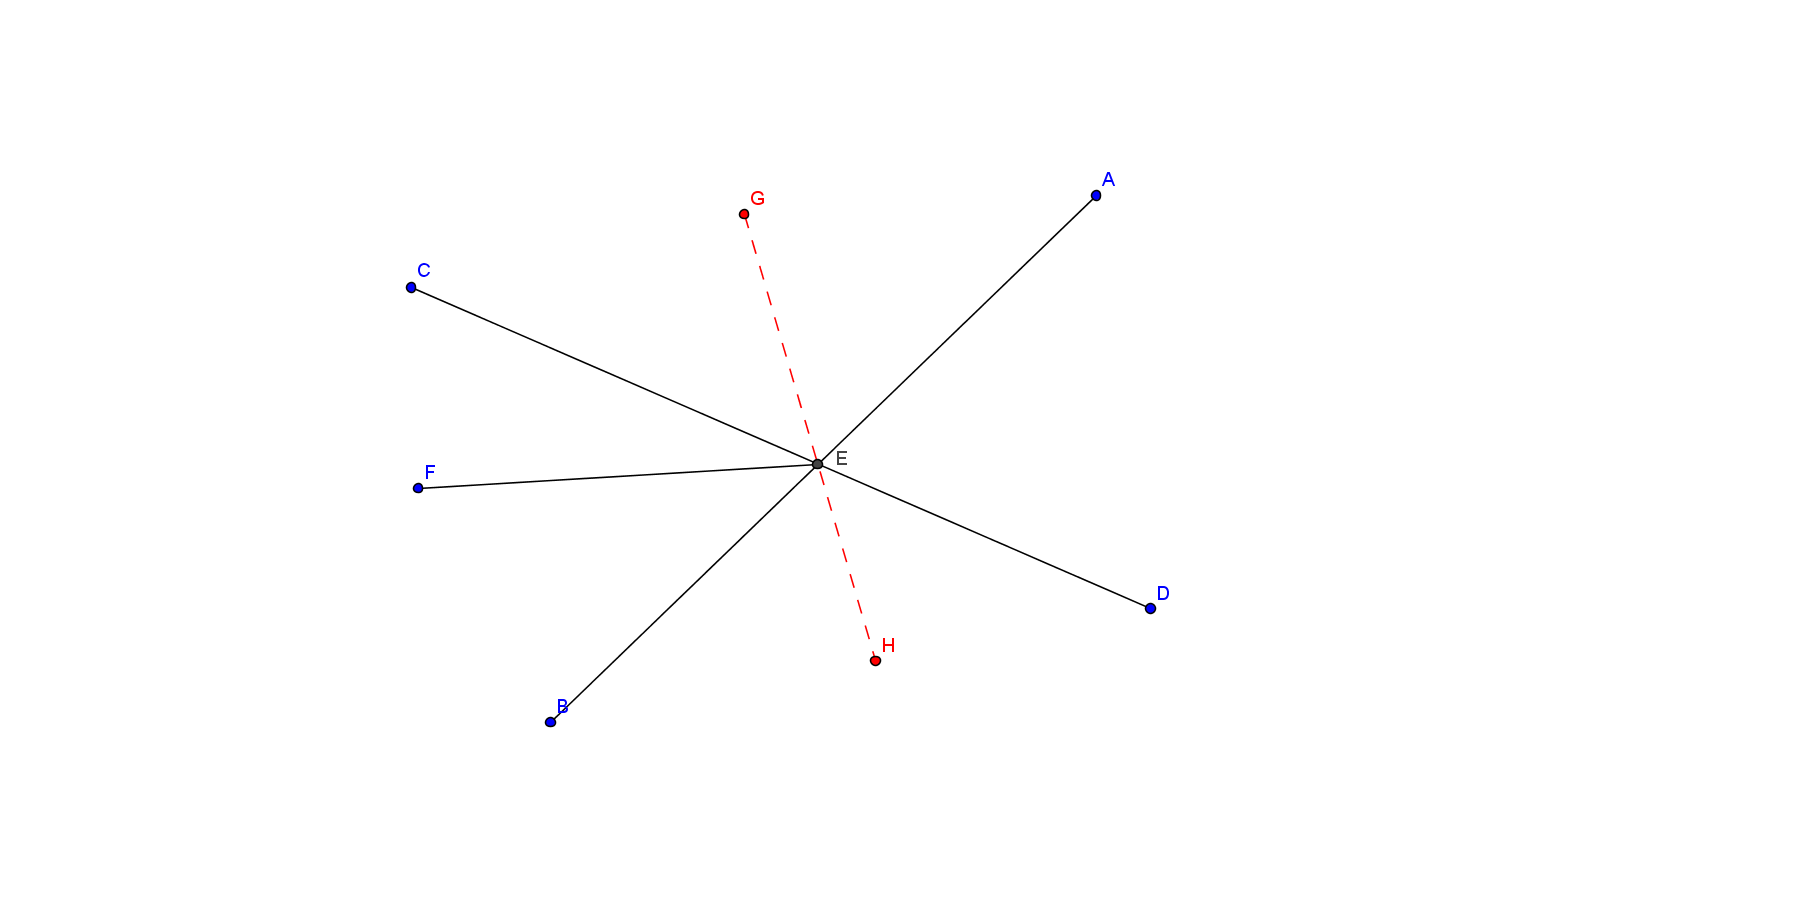
\includegraphics[width=1\textwidth]{rem_dupl}
		\caption{Example on duplicates removal}
		\label{fig:rem_dupl}
	\end{figure}
	before adding the new fracture (the red one), the graph has 5 edges and 6 vertices. Looping on the edges, the algorithm correctly detects one intersection with each edge, but there is only one intersection point, E, and no edge has to be modified by the insertion of the new fracture, therefore all the "duplicates" are discarded but one. Note that this happens just in case of multiple intersections of type "Told" or "common extreme". \\
	Now the vector is ready to be processed. We start passing  \texttt{src} and the first struct of the vector to the function \texttt{refine\textunderscore graph()}: this function performs different actions depending on the intersection type; the common goal is to resolve all the changes due to the insertion of the new fracture and related to that specific segment. The function returns as output the vertex descriptor corresponding to the just created vertex in correspondence of the first intersection point; this descriptor will be passed as source in \texttt{refine\_graph()} at the next iteration together with the second intersection struct in the vector. This procedure goes on until the end of the intersection vector is reached; at the end, the vertex descriptor returned by the last call to \texttt{refine\textunderscore graph()} is connected to \texttt{tgt}. \\
	In case of partial or total overlapping between the new fracture and an existing edge, a conflict between the corresponding edge properties happens: it is up to the user to decide how to solve it, and this is possible passing as optional parameter to \texttt{create\textunderscore graph()} a lambda function \texttt{update\textunderscore edge\textunderscore properties()} which will be used inside \texttt{refine\textunderscore graph()} to merge old and new properties. The default behaviour is simply to keep the old property, totally discarding the new one.
	
	\subsubsection{A simple example}
	This example refers to figure \ref{fig:example_algo} and it aims at illustrating how the algorithm works.
	\begin{figure}
		\centering 
		\includegraphics[width=1\textwidth]{example_algo}
		\caption{Fracture in red is going to be added to the graph}
		\label{fig:example_algo}
	\end{figure}
	We consider the insertion of the fifth fracture (e): the previous four (a,b,c,d) have been already added and the graph they created is made of 8 vertices and 6 edges (AE, BE, CE, DE, FE, GH).  
	Since the extremities of the new fracture have coordinates different from all the other existing points, two new vertices I and J are created. Looping over the edges in the graph, we obtain a vector of six intersection structs; we reorder it and we remove four duplicates in point E (see table \ref{tab:table1}).
	Now we are left with a vector of two components: first of all we pass to \texttt{refine\textunderscore graph()} the vertex descriptor I (which is the source of the new fracture) and the first intersection struct (related to point E); being the intersection of type T\textunderscore old, this function simply adds an edge between I and E and returns as next source E. At the second step, \texttt{refine\textunderscore graph()} takes as input the current source (i.e. the output of the previous call to the function, E in this example) and the second intersection struct: in case of overlap\textunderscore outside the source is connected to the first intersection (EH), the properties of the old edge (HG) are updated and the second intersection is connected with the target (GJ). In conclusion, the insertion of this new fracture led to the creation of three new edges (all labelled with letter e in order to keep track of the fact they all are part of the fifth fracture) and to the property update of an existing edge.
	\begin{table}[h!]
		\centering
		\label{tab:table1}
		\begin{minipage}{.5\textwidth}
			\centering
			\begin{tabular}[t]{ccc}
				\toprule
				Int. edge & Type & Int. point(s)\\
				\midrule
				AE & T\textunderscore old & E\\
				BE & T\textunderscore old & E\\
				FE & T\textunderscore old & E\\
				GH & overlap\textunderscore outside & \textbf{G and H}\\ 
				DE & T\textunderscore old & E\\		
				CE & T\textunderscore old & E\\
				\bottomrule
			\end{tabular}
			\caption*{Initial setting}
		\end{minipage}%
		\begin{minipage}{.5\textwidth}
			\centering
			\begin{tabular}[t]{ccc}
				\toprule
				Int. edge & Type & Int. point(s)\\
				\midrule
				AE & T\textunderscore old & E\\
				BE & T\textunderscore old & E\\
				FE & T\textunderscore old & E\\
				DE & T\textunderscore old & E\\		
				CE & T\textunderscore old & E\\
				GH & overlap\textunderscore outside & \textbf{H and G}\\ 
				\bottomrule
			\end{tabular} 
			\caption*{Ordered}
		\end{minipage}%
		
		\begin{minipage}{0.5\textwidth}
			\centering
			\begin{tabular}[t]{ccc}
				\toprule
				Int. edge & Type & Int. point(s)\\
				\midrule
				AE & T\textunderscore old & E\\
				GH & overlap\textunderscore outside & G and H\\ 
				\bottomrule
			\end{tabular}
			\caption*{Ordered and without duplicates\\(Final setting)}
		\end{minipage}
		\caption{Simplified representation of the intersection vector}
	\end{table}		
	
	\subsubsection{A more complex example}
	In the file \texttt{test\_all\_int\_cases.txt} we put a list of fractures with no property associated: the main goal of this example is to show that the code performs correctly whatever is the intersection type it has to handle. Indeed, the sequence of fractures is built in such a way that almost every intersection type appears during the construction of the graph. 
	\begin{figure}
		\centering 
		\includegraphics[width=1\textwidth]{graph_building_process}
		\caption{Fracture in red is going to be added to the graph}
		\label{fig:graph_steps}
	\end{figure}
	In figure \ref{fig:graph_steps} we show how the graph is built step by step, one fracture at a time.
	
	\subsubsection{Handling "real" data}
	In order to test our algorithm, professor Formaggia provided us two lists of fractures. The input files' formats were different, so we implemented two specific readers, inherited by our \texttt{BGLgeom::reader\_ASCII} class, to acquire the fractures' extremities and their properties in the right way. \\
	The source code is in file \texttt{main\_fractures.cpp} and the graphical result are shown in figure \ref{fig:plots_real_fractures}.
	\begin{figure}
		\centering
		\begin{subfigure}{.5\textwidth}
			\centering
			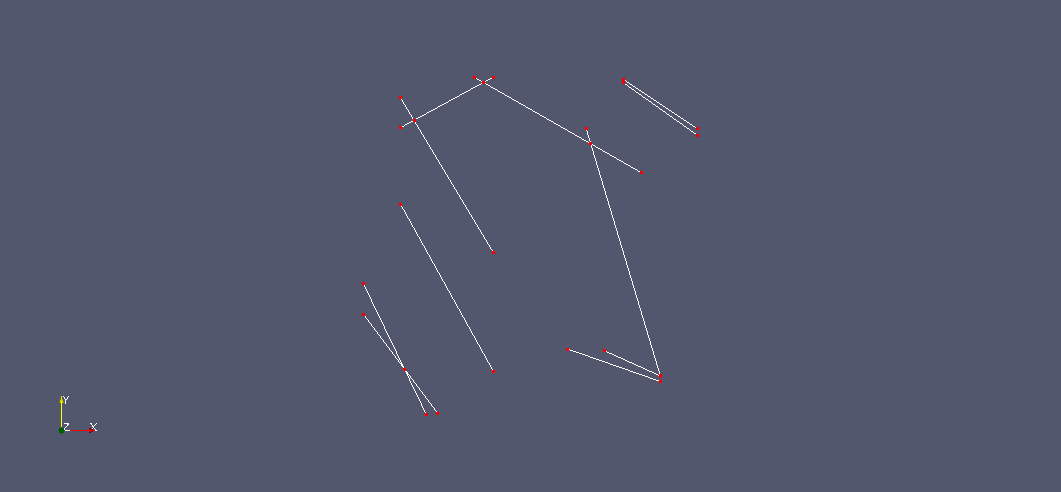
\includegraphics[width=.9\linewidth]{graph1}
  			\caption*{input file: fractureElevenVF.dat}
		\end{subfigure}%
		\begin{subfigure}{.5\textwidth}
			\centering
			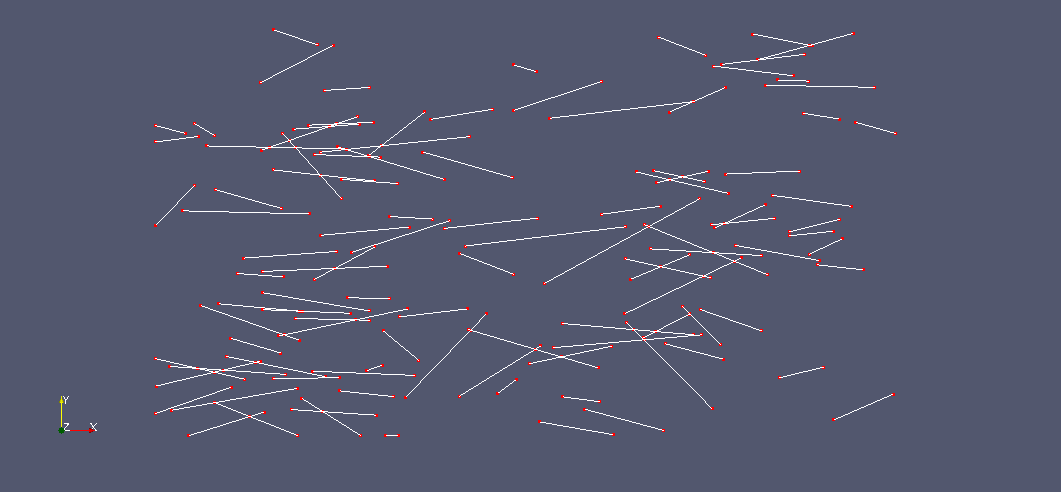
\includegraphics[width=.9\linewidth]{graph2}
			\caption*{input file: fractures.txt}
		\end{subfigure}
		\caption{plots of resulting graph on Paraview}
		\label{fig:plots_real_fractures}
	\end{figure}
	
	\subsection{Coupled problems on one-dimensional networks with application to microcirculation}
	
	\subsubsection{Mathematical formulation}
	We present a prototype model for fluid transport in a permeable biological tissue perfused by a capillary network. 
	The domain where the model is defined is composed by two parts, $\Omega_t$ and $\Omega_v$ (where $t$ stands for \textit{tissue} and $v$ stands for \textit{vessel}), denoting the interstitial volume and the capillary bed respectively.
	We assume that the capillaries can be described as cylindrical vessels and  $\Lambda$ denotes the centerline of the capillary network. The capillary radius, $R$, is for simplicity considered to be constant.  We decompose the network $\Lambda$ into individual branches $\Lambda_i$. Branches are parametrized by the arc length $s_i$; a tangent unit vector $\boldsymbol \lambda_i$ is also defined over each branch, defining in this way an arbitrary branch orientation. In particular, the domain $\Omega_f$ can be split into cylindrical branches $\Omega_i$ defined as follows
	\begin{align*}
	\Omega_i = & \{ \xx \in \R^3; \ \xx = \ss + \rr\}; \\
	\ss \in \Lambda_i = & \mathcal{M}_i(\Lambda^\prime \subset \R^1)\}; \\
	\rr \in \mathcal{D}_{\Lambda_i}(\ss,R) = & \{ r \nn_{\Lambda_i}; \ r\in(0,R)\};
	\end{align*}
	where $\mathcal{M}_i$ is a mapping from a reference domain $\Lambda^\prime$ to the manifold $\Lambda_i \subset \R^3$ and $\nn_{\Lambda_i}$ denotes a unit normal vector to $\Lambda_i$. We denote with $\Gamma_i$ the lateral surface of $\Omega_i$. 
	
	\begin{figure}
		\centering
		\includegraphics[width=0.7\linewidth]{"3d-1d domain"}
		\caption[Fig. 1]{On the left the interstitial tissue slab with one embedded capillary; on the right reduction from 3D to 1D description of the capillary vessel.}
		\label{fig:3d-1d-domain}
	\end{figure}	
	
	The physical quantity of interest is the concentration of transported solutes c. It is defined as a field depending on time t and space, being $x \in \Omega$
	the spatial coordinates. Furthermore, we denote with the subscript v their restriction to the capillary
	bed (vessels), and with t the restriction to the interstitial tissue. The derivation of our model stems
	from fundamental balance laws regulating the flow in the capillary bed, the extravasation of plasma
	and solutes and their transport in the interstitial tissue.	
	\newline\newline
	Mass transport is modeled by means of diffusion equations, both in the tissue and in the capillary bed. Furthermore, we want to couple the two problems with a leakage in the vessel walls; then, under the assumption that capillaries
	can be modeled as cylindrical channels, the magnitude of the mass flux exchanged per unit length
	between the network of capillaries and the interstitial volume at each point of the capillary vessels
	is the following:
	\begin{equation}
	J := k_i \left( c_v - c_t\right)  \quad \text{on } \Gamma_i,
	\end{equation}
	being $k_i$ the permability of the vessel wall $\Gamma_i$. \\
	Finally, using this notation, the problem becomes:
	\begin{align}
	\label{eq:fullProblem3D}
	\begin{cases}
	- \Delta c_t = 0 &\text{ in } \Omega_t,\\
	\nonumber
	- \Delta c_v = 0 & \text{ in } \Omega_v,\\
	\nonumber
	-\nabla c_t \cdot n_t = \kappa_i \left( c_t - c_v \right) & \text{ on } \Gamma_i,\\
	\nonumber
	-\nabla c_v \cdot n_v  = \kappa_i \left( c_v - c_t \right) & \text{ on } \Gamma_i,\\
	\nonumber
	\nabla \cdot c_t = 0 & \text{ on } \partial \Omega_p \setminus \cup_{i=1}^N \Gamma_i,\\
	\nonumber
	c_v = g & \text{ on } \Gamma_{inflow}\\
	\nonumber
	\nabla \cdot c_v = 0 & \text{ on } \Gamma_{outflow}
	\end{cases}
	\end{align}
	
	The problem on $\Omega_v$ is a prototype of flow or mass transport problem in a network of cylindrical channels, surrounded by the domain $\Omega_v$ where another flow and transport problems will be defined, according to porous media equations. It is assumed that the interface between these regions is permeable, namely it is crossed by a normal flux proportional to $\kappa_i \left( u_t - u_v \right)$.\\
	The boundary of $\Omega_v$ is divided as follows: $\partial \Omega_v =\Gamma_{inflow} \cup \Gamma_{outflow} \cup_{i=1}^N \Gamma_i $; then, we impose boundary conditions on $\Omega_v$ such that the mass goes from $\Gamma_{inflow}$ to $\Gamma_{outflow}$.\\
		
	Applying model reduction techniques, the equations defined on the network of inclusions $\Omega_v$ can be restricted to the one dimensional network $\Lambda$. Differentiation over the branches is defined using the tangent unit vector as ${\partial_{s_i}} = \nabla \cdot \pmb{\lambda}_i\,$ on $ \Lambda_i$, i.e. ${\partial_{s_i}}$ represents the projection of $\nabla$ along $\boldsymbol \lambda_i$. \newline	
	As a result, the 3D-1D counterpart of the problem becomes
	\begin{equation}\label{eq:redweak3D1D}
	\begin{cases}
	a(c_t,q_t) + b_\Lambda(\bct,\bqt) = b_\Lambda(c_v,\bqt) & \forall q_t \in H^1_0(\Omega_t),
	\\
	A(c_v,q_v) + b_\Lambda(c_v,q_v) = b_\Lambda(\bct,q_v) + \mathcal{F} (q_v) & \forall q_v \in H^1_0(\Lambda),
	\end{cases}
	\end{equation}
	where $c_v,q_v \in H^1_0(\Lambda)$ denote trial and test functions relative to the weak reduced problem, with the following bilinear forms:
	%
	\begin{equation*}
	a(w,v) = (\nabla w,\nabla v)_{\Omega}, 
	\quad
	A(w,v) = \sum_{i=1}^N (\nabla_{\Lambda_i} w, \nabla_{\Lambda_i} v)_{\Lambda_i}, 
	\quad 
	b_\Lambda(w,v) = \sum_{i=1}^N \kappa_i (w,v)_{\Lambda_i}.
	\end{equation*}
	A central role in equation \eqref{eq:redweak3D1D} is played by the restriction operator $\overline{(\cdot)}$ that is defined as
	\begin{equation*}
	\overline{w}^{(i)} = 
	\frac{1}{|\partial\mathcal{D}_{\Lambda_i}|} \int_{\partial\mathcal{D}_{\Lambda_i}} w|_{\Lambda_i \times \partial\mathcal{D}_{\Lambda_i}}\,dr\,d\theta\,.
	\end{equation*}
	
	\subsubsection{Code implementation and results}
	We use a C++ code that exhibits one-to-one correspondence with respect to the
	mathematical models derived. Specifially, we assemble the generic linear
	system using GetFEM++, an open-source general-purpose finite element library. For the results presented in this report we applied the direct solver SuperLU 3.03 to solve the monolithic linear system.
	The code has been written by Stefano Brambilla and it is part of another PACS project; the code can be found at the following GitHub page: \texttt{https://github.com/stefano-brambilla-853558/MANworks}.
	\newline\newline
	The code needs to read from a file containing the structure of the network: so we first developed a Matlab script to generate the coordinates of all the vertices of a network with successive bifurcations on orthogonal planes. We used our library to read this file and construct the relative graph, then we created a 1D mesh on each edge, and in the end we used the graph and its properties to generate the \texttt{diffusion\_network.pts} file, containing the details of the 1D mesh and of the boundary conditions.
	\newline
	The results show that the mass diffuses into the network and then flows thwrough the vessel walls into the surrounding tissue.
	
	\begin{figure}[h]
		\centering
		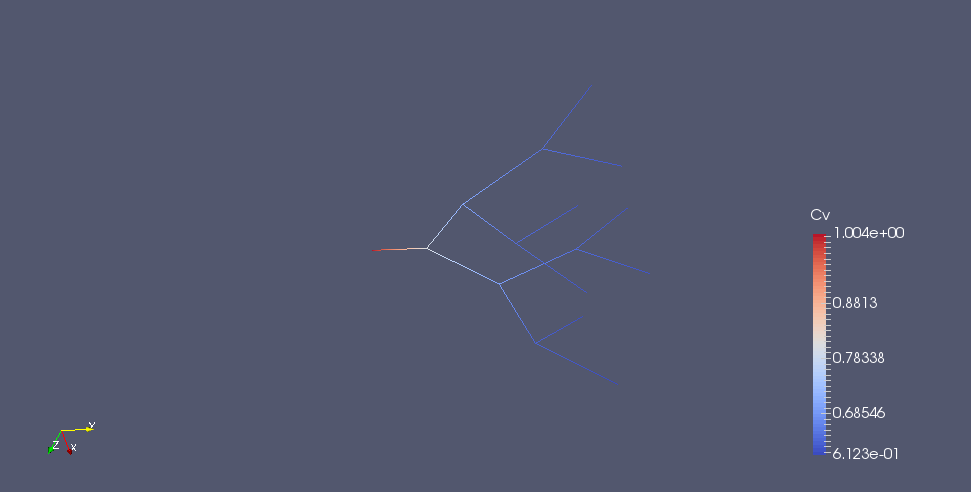
\includegraphics[width=0.92\linewidth]{cv}
		\label{fig:cv}
	\end{figure}
	
	\begin{figure}[!h]
		\centering
		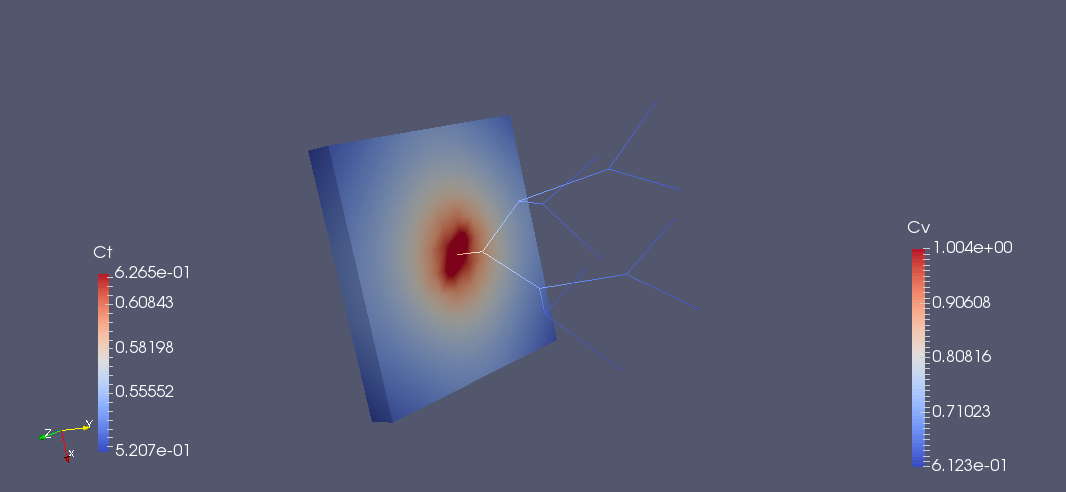
\includegraphics[width=0.92\linewidth]{ct1}
		\label{fig:ct1}
	\end{figure}
	
	\begin{figure}[!h]
		\centering
		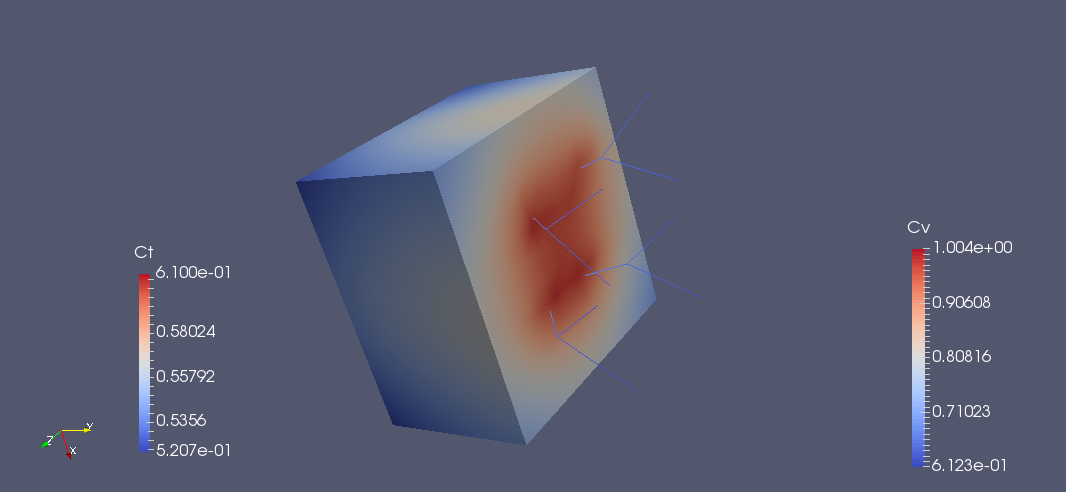
\includegraphics[width=0.92\linewidth]{ct2}
		\label{fig:ct2}
	\end{figure}
	
	\begin{figure}[!h]
		\centering
		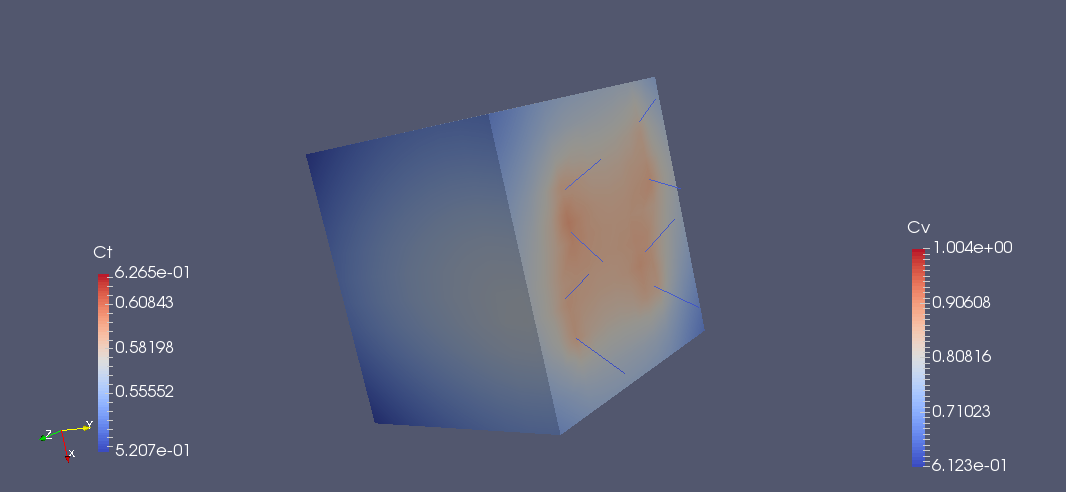
\includegraphics[width=0.92\linewidth]{ct3}
		\label{fig:ct3}
	\end{figure}
	\newpage
	\section{Bibliography}
	\begin{itemize}
		\item user guide malloppone che ci siamo letti su BGL
		\item www.stackoverflow.com
		\item https://www.fim.uni-passau.de/fileadmin/files/lehrstuhl/sauer/geyer/SplinesinIndustry.pdf, rigurado interpolazione bspline
		\item http://www.boost.org/doc/libs/1\_61\_0/libs/graph/doc/, sito web della BGL
		\item http://www.gnu.org/software/make/manual/make.html, cose varie su makefile (usato solo per qualche dettaglio)
		\item http://eigen.tuxfamily.org/dox, documentazione su Eigen
		\item http://www.stack.nl/~dimitri/doxygen/manual/index.html, documentazione di doxygen (ma non saprei neanche se metterla)
		\item http://www.vtk.org/Wiki/VTK/Examples
	\end{itemize}

	\section{Acknowledgements}
	We would like to thank our mate Stefano for his support, both practical and moral, in our PACS project. In particular, since he is working on another PACS project on that topic, he helped us a lot in writing the source code for the vascular microcirculation application, and he also gave us large support in writing the report part concerning that application, expecially the mathematical formulation.
	\newline\newline
	We want also to thank Dr. Pasquale Africa for its technical support when nothing was compiling on our virtual machine. Always helpul, he gave us a lot of advice on how to write a good Makefile and some suggestions on how to design our code and the library structure.
\end{document}
